\chapter{Resultados}

% Falar da implementação (PyTorch)

Foi feita a implementação do
método de Síntese de Textura
usando a abordagem das matrizes
de Gram. 
Para isso foi utilizada 
a linguagem Python com a
biblioteca PyTorch.
O PyTorch reúne uma série de
funções que facilitaram
a implementação do método.
As principais foram: implementação
nativa da rede VGG-19, operações
aritméticas aceleradas na GPU,
cálculo automático de gradiente,
e implementação do método de
otimização L-BFGS.

% Escolha de textura

A primeira ideia era escolher um
conjunto de textura de resolução
$128 \times 128$ e tentar gerar
imagens de $256 \times 256$ pixels.
Foram escolhidos um conjunto de
diferentes tipos de texturas 
para explorar o comportamento
do algoritmo.

% Mostrar os resultados

%Em todos os testes a primeira imagem é
%a amostra, e as seguintes são passos (não
%necessariamente consecutivos) do
%algoritmo de otimização.

\begin{figure}[!ht]
	\centering
	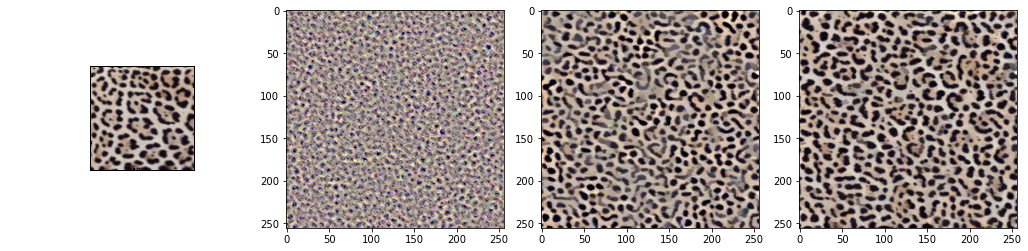
\includegraphics[width=\linewidth]{files/assets/results/result2.png}
	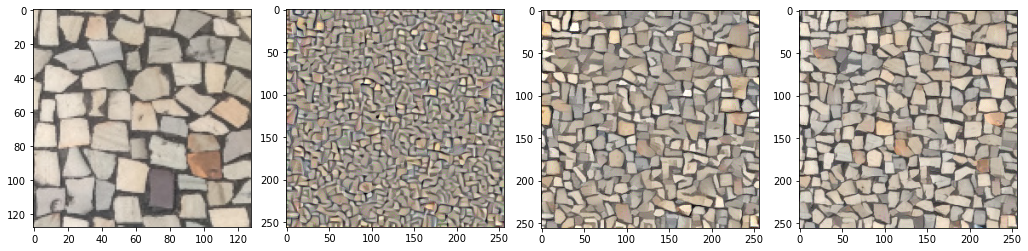
\includegraphics[width=\linewidth]{files/assets/results/result5.png}
	\caption{Teste com texturas mais caóticas. A primeira imagem
	é a amostra, e as seguintes são sínteses a medida que
	o número de iterações cresce.
	No processo, a escala dos objetos se mantém, portanto o resultado
	terá quatro vezes mais informação.}
	\label{img:preview}
\end{figure}


\begin{figure}[!ht]
	\centering
	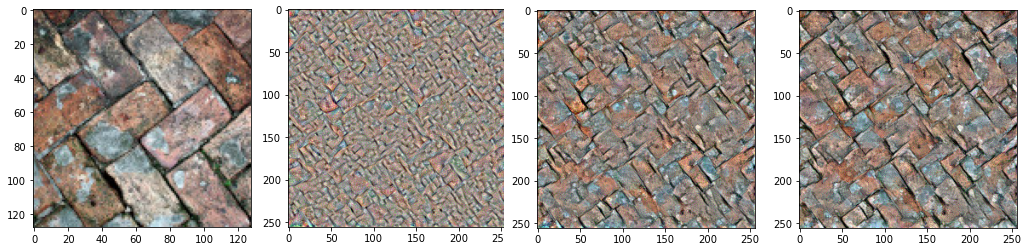
\includegraphics[width=\linewidth]{files/assets/results/result1.png}
	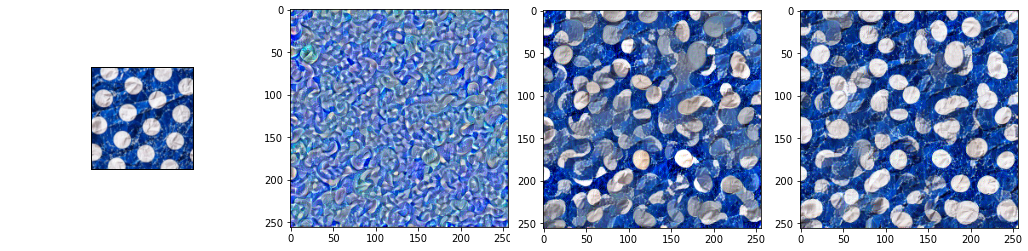
\includegraphics[width=\linewidth]{files/assets/results/result3.png}
	\caption{O método não funciona bem em textura com 
	estrutura regular global, ele dá preferência por
	estruturas locais. }
	\label{img:preview}
\end{figure}



\begin{figure}[!ht]
	\centering
	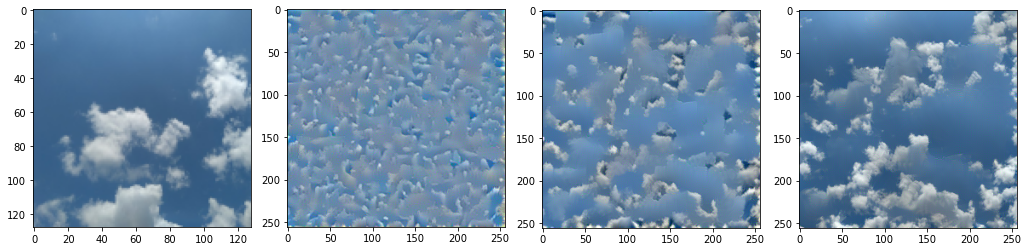
\includegraphics[width=\linewidth]{files/assets/results/result4.png}
	\caption{Nuvens apresentam uma estrutura caótica
	ideal para esse método.}
	\label{img:preview}
\end{figure}
% Falar da animação

Ao gerar algumas texturas, notou-se que durante
o processo de otimização a imagem fica preza em 
uma estrutura específica. Com isso foi pensado
em adicionar ruído na imagem em intervalos de iterações
para forçar a mudança do ponto de convergência.
Isso gerou um resultado interessante de movimentar
suavemente a textura a cada aplicação do ruído.

\begin{figure}[!ht]
	\centering
	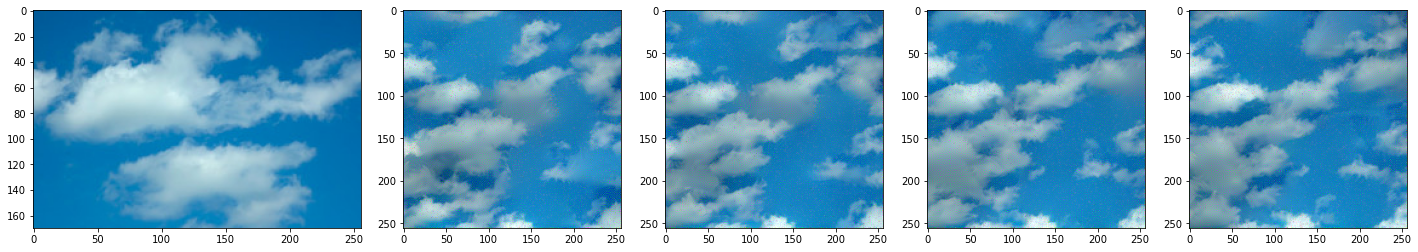
\includegraphics[width=\linewidth]{files/assets/results/result6.png}
	\caption{A terceira imagem foi gerada a partir da adição de ruído
		na segunda, assim como da terceira pra quarta e da quarta pra
		quinta. 
		Com isso, as quatro imagens geradas aparentam o processo
	que aparenta movimento nas nuvens.}
	\label{img:preview}
\end{figure}

% Teste com imagens não textura

Não é preciso se limitar a texturas com
esse tipo de implementação. É possível verificar
o que acontece no resultado com imagens não textura.

\begin{figure}[!ht]
	\centering
	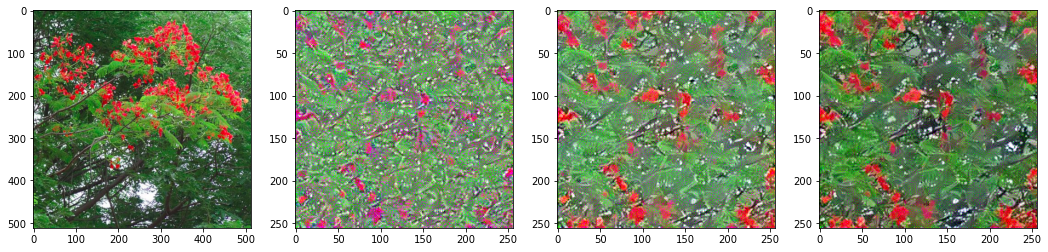
\includegraphics[width=\linewidth]{files/assets/results/result7.png}
	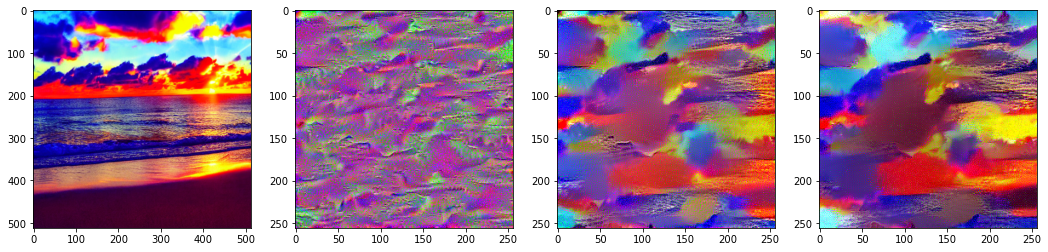
\includegraphics[width=\linewidth]{files/assets/results/result8.png}
	\caption{Teste com imagem não textura. A informação espacial da imagem foi perdida,
	mas cores e formas prevalecem.}
	\label{img:preview}
\end{figure}

% Style transfer

% Não fica restrito a textura

% Multiescala?

\chapter{Conclusão}

Esse trabalho mostrou o quanto
pode ser difícil a tarefa de
processamento e síntese
de texturas e imagens no geral,
e o quanto foi preciso andar
para chegar nos avanços que
existem hoje.
Uma grande quantidade de trabalhos
são publicados todos os anos
na área, cada um tentando
encontrar uma maneira nova de
melhorar a solução do problema.

Redes Neurais e Deep Learning
vêm se mostrando ferramentas
bem poderosas para o trabalho com imagem.
Redes Convolucionais pré-treinadas
para a detecção de objetos
oferecem uma excelente métrica
perceptual, abrindo caminho para
diversos novos trabalhos.
O aprendizado automático
de representações facilita
o trabalho de criar aplicações
de processamento e síntese de imagens,
mas a disponibilidade de dados
e de processamento ainda pode ser
um problema.

% A principal vantagem de
% Redes neurais é aprender
% métricas perceptuais

% Redes neurais pre-treinadas
% não são apenas para classificação

Ferramentas para trabalhar
com Machine Learning como o
PyTorch vêm se mostrando
mais poderosas
a cada dia, oferecendo
facilidades para trabalhar 
com grandes quantidades de dados,
além de fácil acesso à GPU,
que melhora bastante a velocidade
de operações aritméticas.
Essas ferramentas também 
contam com sistemas de cálculo automático
de gradiente, o que torna o trabalho
de otimização mais fácil e
menos suscetível a erros.




% PyTorch é uma boa ferramenta
% de deep learning, GPU acelera


%\section{Perspectivas}
% Definir depois